\clearpage
\section{Questions, hypotheses and findings}

The questionnaire starts with a short paragraph recalling the European debt
crisis that started in 2010, and the \textit{Memoranda of Understanding}
that Greece, Spain, Portugal, Ireland and Cyprus signed with the European
Union, the European Central Bank and the International Monetary Fund that  
established financial aid combined with economic adjustment. We refer to
these contracts as \textit{aid\&reform} programs. 

In a first question we asked the respondents for each EMU member whether
this was a program country or not, where a respondent could answer "yes",
"no", or "I don't know". The question has two purposes. First, it provides
information about the aggregate state of information. There are multiple
ways to aggregate the answers from 19 questions.\footnote{%
A very small number of experts found this question imprecisely stated. \emph{%
We omit these replies the statistical analysis of this question?}} We
calculate a simple score:\ we count the number of program countries
correctly identified and deduct the number of wrong answers (both if a
respondent names a non-program country as program country or if the
respondent thinks that a program country did not sign a memorandum). Thus, the maximum score participants can obtain is 5, the minimum score -19. On
average, these numbers are

\begin{equation*}
\begin{tabular}{lll}
& Experts & Non-Experts \\ 
from borrower countries & $%
\begin{array}{c}
2.48 \\ 
(2.62)%
\end{array}%
$ & $%
\begin{array}{c}
1.10 \\ 
(2.74)%
\end{array}%
$ \\ 
from lender countries & $%
\begin{array}{c}
.78 \\ 
(3.50)%
\end{array}%
$ & $%
\begin{array}{c}
-.96 \\ 
(3.59)%
\end{array}%
$%
\end{tabular}%
\end{equation*}%
In the aggregate, experts were better informed than non-experts, but even
among the non-experts, the European debt crisis is an event that left
considerable memories. 

We also use these data as explanatory variables in the multivariate
regressions. In particular, we might use the score as the
individual's state of correct memory, and generate a dummy variable that is
1 if the individual correctly remembers the role of his or her own country,
and zero otherwise. 

We now turn to the questions that report possible collective
self-serving memory biases. We first address the question whether country
origin matters for respondents' opinions about the \textit{reasons} for why lender countries wanted to engage in the credit relationship. 
\begin{figure}[h!]
\caption{Reasons of the lender countries for entering the rescue program}
    \centering
    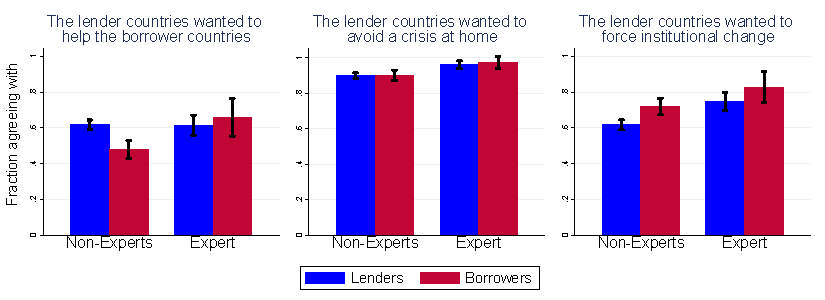
\includegraphics[scale=1.2]{graph2.pdf}
  
    \label{fig:my_label}
\end{figure}

The mean denotes the share of survey participants who stated that they either strongly or slightly agreed with the statement. We exclude all participants who answered with I don't know.  

The nation-serving hypothesis is:\ respondents from borrower countries tend
to agree less frequently than respondents from lender countries 
that the lender countries wanted to help. They agree more that
the lender countries wanted to help themselves, and they agree more 
often that the lender countries wanted to force institutional change on the
crisis countries.\textit{\ }

Data are largely in line with this hypothesis. Compared to
non-expert respondents from the lender countries, the non-expert respondents
from the borrower countries tend to agree less that the
lenders wanted to help the borrower countries. 
The difference in assessments between
non-expert respondents from the two groups are large and highly
significant for the aspect of reforms. It is conceivable that
many non-expert respondents in the borrower countries were suspicious that
the lender countries had an institutional-reform agenda that goes beyond the
idea of helping each other. There is also some disagreement concerning
this circumstance in the expert sample. The differences, however, do not turn out to be statistically significant. 


This insight will be useful for the
interpretation of the answers to questions where we asked the respondents
about feelings of guilt, being exploited, disappointed, or feeling inferior,
and about the friendship-building capacity of the aid\&reform programs.

It might be surprising that the country origin of experts does not have a
similar impact on their response. We can only speculate about the reason for
this discrepancy, but it seems probable that experts, apart from simply being
better informed, often identify less with their own countries of origin and have 
a more cosmopolitan orientation. (At
least, this was the hypothesis that guided us to subject non-expert
nationals from the different countries to the same survey). Therefore, the
forces for developing a nation-bias might be less strong for experts than for non-experts. 

\begin{figure}
    \centering
      \caption{Driving Force and Beneficiaries}
    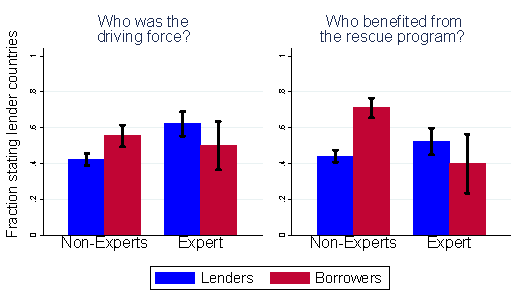
\includegraphics[scale=1.2]{graph3.pdf}
  
    \label{fig:my_label}
\end{figure}
Question 3 is similar to question 2 and asks about underlying motivations
and intentions. Question 4 asks about the beneficiaries of the aid\&reform
programs.  We
turn now to the next two questions. As we
will see, the difference in nation-bias is a more systematic pattern. Both questions show very similar patterns for non-expert
respondents, depending on whether they are from borrowing countries or from
lender countries. They show large and significant nation-biases. Non-expert respondents
from borrowing countries tend to see the lender countries as the main
motivators for these programs, in any case, more than respondents from the
borrower countries. This result is reminiscent of the results on
self-serving memories from private informal lending as in Desz\"{o} and L%
\"{o}wenstein (2012), where there is a tendency to assign the initiative\
for such contracts to the respective other side of the credit relationship. 

Non-expert respondents from borrowing and lending countries also differ in
their perceptions of who mainly benefited from the aid\&reform programs. The
bias tends to assign the benefits more to the counterparty group:\
respondents from borrower countries think more often than respondents from
the lender countries that the lender countries are the major beneficiaries. These numbers
suggest that there is a nation-serving bias. 

If we look at the responses of experts, we find no significant country-group
bias. Whether an expert is originally from a borrower country or a lender
country does not systematically affect their assessments about the
motivations driving the aid\&reform programs, nor their assessments about
who was the main beneficiary. \footnote{It is important to note that 98 percent of experts also works in their country of origin }Interestingly, the results show that the
nation-serving bias was reversed with experts from lender country agreeing more, on
average with the statements outlined above. However, these results do not turn out to be significant.

We now turn to questions addressing how the different groups of respondents
assess the implications of the aid\&reform programs for feelings among the
populations in the group of borrower countries and in the group of lender
countries. The respondents' perceptions might be formed by direct
observations in the countries or media reports, but their views about the
reasons and motivations for the aid\&reform programs and their views about
who actually benefited from these programs should correlate with their
assessments, and might actually cause their beliefs about these feelings. 

The first set of questions addresses the population in the group of borrower
countries. We ask whether respondents think that the rescue experience might
have caused feelings of \textit{guilt}, feelings of \textit{being
exploited}, and/or feelings of \textit{inferiority}. The answers to these
questions, and possible differences for respondents from lender countries or
from borrower countries do not have an immediate interpretation in terms of
nation-serving collective memory biases, but might rather be the outcomes of
such biases. Consider a citizen in the borrower country, say Greece. This
citizen will (supposedly)\ truthfully state what he or she believes what the
co-citizens in Greece feel. For instance, whether or not they feel guilt.
This feeling might, among other factors, be a result of a (potentially
nation-serving) view about how the crisis came about, and how Greece
addressed the crisis. If the views about reasons/motivations and the
distribution of benefits for the aid\&reform programs are self-serving, then
the Greek citizen might not see any reason for guilt:\ the crisis was just
bad luck, Greece was forced to take up more than the right amount of
(painful) reforms, and the benefits from these measures went elsewhere.
Hence, the Greek population might not see any reason to feel guilty.
Assessing the positions of respondents in the lender countries, these might
think that the crisis was caused by poor pre-crisis politics in Greece, that
Greece got a lot of assistance (see the previous questions) and resisted to
follow the Troika advice on necessary reforms for recovery. What does this
perception mean for beliefs about guilt? The respondent from the lender
country might think:\ if I were them, for what they have done, I would feel
guilty. The respondent might also have second-order beliefs.\ The respondents
might understand that the citizens in Greece perceived matters in a
nation-serving way and therefore will not feel guilty. While this modifies
possible expected outomes, overall this reasoning points at a
borrower-country bias towards not agreeing that the citizens of these
countries feel guilty. 


\footnote{Our findings can also be interpreted in an alternative way.  Having a self-serving or nation-serving bias might make individuals oblivious to
the way policies are received in other countries. 
\cite{dezso} refer to this phenomenon as having a ``blind spot" regarding the other party's 
feelings and emotions. The hypothesis on the existence of such a ``blind spot" is confirmed in our findings.
Citizens from lender countries are more likely to agree that they felt guilty, exploited and/or inferior as a 
consequence of the rescue program. The largest difference between lender and borrower countries occurs with regards to feeling exploited.
78 percent  of citizens from borrower countries state that they felt exploited due to the rescue program while only 61 percent of lender countries
agree to this statement. 
}

%Similar reasons might let us suspect that the respondents from the lender
%countries are more inclined to think their population feels exploited, or
%feel inferior (in the sense of humiliated). Figure xxx shows the answers.
%First statistics negate the existence of a blind spot among borrowers about the feelings
%from citizens to lender countries. 

\begin{figure}
    \centering
    \caption{Emotions of the borrower countries}
    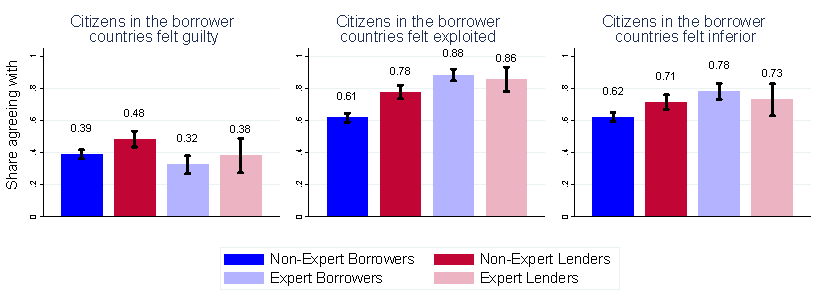
\includegraphics[scale=1.2]{graph5_1.pdf}
    
    \label{fig:my_label}
\end{figure}

We might expect that experts have a view on these questions that is not, or
less coloured by their countries of origin, such that we would not find much
difference in the responses of participants who originated in the borrower
countries and those of participants who originated in the lender countries.


Similar questions assess the perceptions in the different groups about the
feelings in the lender countries. In particular, we asked them whether they
agree or disagree on that the aid\&reform programs made the citizens in the
lender countries feel exploited and disappointed. Again here, the results
might be interesting on their own. While the non-experts in the lender
countries might convey an adequate picture about their own feelings, the
perceptions about these lender-country feelings by the respondents from the
borrower countries might be distorted for several reasons. If they believe
that the lender countries are the true winners of these programs and that
this is how the citizens in these countries feel about it, they should agree
less to the ideas that citizens in lender countries feel exploited and
disappointed. If, however, they have second-order beliefs and can
successfully place themselves in the shoes of lender-country citizens, they
might understand that their beliefs about how the crisis came about and who
benefited from the programs are quite different, and they might correctly
assess their true feelings of being exploited and disappointed. Overall,
however, we might expect that the lender-country respondents agree more
frequently than the borrower-country respondents to the possibly negative
feelings in lender countries:

\begin{figure}[h!]
    \centering
       \caption{Emotions of the lender countries}
    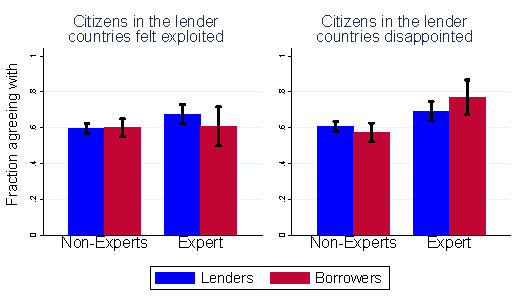
\includegraphics[scale=1.2]{graph5_2.pdf}
 
    \label{fig:my_label}
\end{figure}

Again, we can compare non-experts and experts. We do not observe any divergence 
between borrower and lender country citizens in the assessment of these statements in
both the expert and the non-expert sample. 

The findings here are interesting from the perspective of possible
nation-serving collective memories. They also indicate that the populations
in both groups of countries believe that the \textit{aid\&reform programs} triggered
bad feelings in both groups of countries. A large share of the respondents
thinks that citizens in borrower countries feel guilty, exploited, and
inferior, and a large share of respondents also thinks that citizens in
lender countries feel disappointed and exploited as well. This actually
leads to a final question on the feelings in the two country groups that
asks whether the \texti{aid\&reform programs} strengthened friendship between the
citizens in the Eurozone. 

As is well-known from the theory of groups and conflict theory, an important
means to overcome negative attitudes and mutual spite between groups is that
the groups jointly master a major task which none of them could have
mastered in isolation. The European debt crisis had the potential to be 
such a task. It might have strengthened friendship between these groups.
However, if both groups have nation-serving diverging biases about what
motivated the crisis and the solution method adopted, and about the
distribution of the benefits and costs of the method adopted, then we might
expect that a large fraction of the respondents of both groups think that
these programs did not strengthen friendship ties. Theory cannot make a
clear prediction here, but the result is, of course, interesting.
\begin{figure}
\centering
\caption{Impact on friendships}
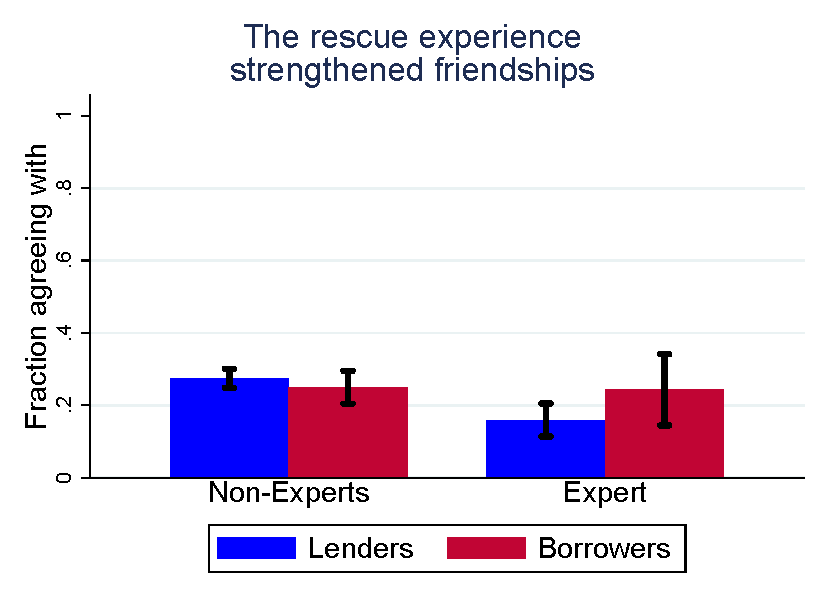
\includegraphics[scale=0.5]{graph5_3.pdf}
\end{figure}

The majority of participants from the expert and non-expert sample disagree that 
the rescue package strengthened friendships.\footnote{Due to a survey error this question was displayed as "The rescue experience strengthened friendship ties between borrower". The fraction of experts who answered this question with "I don't know" lies around 20 percent. This is very much in line with the frequency of "I don't know" responses throughout the survey. Hence, it seems plausible that participants correctly understood the question. } This holds for participants from 
both the expert and the non-expert sample. This finding is also in line with the nation-serving biases
we find throughout the survey. In light of the absence of such a bias among the expert sample 
it seems interesting that the level of agreement in this sample is also quite low. 
This might suggest that although experts might not have and be aware of a nation-serving bias
among citizens from the lender countries they are indeed aware of the consequences of such 
a nation-serving bias. 
\\

The reasoning that discussed possible hypotheses for the answers to
questions 5a-5e suggests that answers to the various questions are likely to
be interdependent. We might expect that individuals in lender countries who
think that the borrower countries pushed for the aid\&reform programs
(questions 2 and 3) also think that these are the main beneficiaries
(question 3), and therefore think that the lender countries feel exploited
and disappointed. The direction of causality for respondents from the lender
countries would be%
\begin{equation*}
\begin{array}{ccccc}
\begin{array}{c}
\text{borrower countries} \\ 
\text{pushed for aid\&reform}%
\end{array}
& \rightarrow  & 
\begin{array}{c}
\text{borrower countries} \\ 
\text{are the main} \\ 
\text{beneficiaries of} \\ 
\text{aid\&reform}%
\end{array}
& \rightarrow  & 
\begin{array}{c}
\text{lender countries} \\ 
\text{feel exploited} \\ 
\text{and disappointed.}%
\end{array}%
\end{array}%
\end{equation*}

Respondents from the borrower countries who think that the lender countries
pushed for the aid\&reform programs, wanted to impose institutional reforms
on them are probably the same who think that the lender countries are the
main beneficiaries, and also the same ones who think that the borrower
countries have been exploited and would not feel guilt, but feel humiliated
("inferiority"?). The direction of causality is%
\begin{equation*}
\begin{array}{ccccc}
\begin{array}{c}
\text{lender countries} \\ 
\text{pushed for aid\&reform} \\ 
\text{and wanted to impose} \\ 
\text{structural reforms}%
\end{array}
& \rightarrow  & 
\begin{array}{c}
\text{lender countries} \\ 
\text{are the main} \\ 
\text{beneficiaries of} \\ 
\text{aid\&reform}%
\end{array}
& \rightarrow  & 
\begin{array}{c}
\text{borrower countries} \\ 
\text{feel exploited}%
\end{array}%
\end{array}%
\end{equation*}

\\
